\documentclass[11pt]{article}
\usepackage[francais]{babel}
\usepackage[utf8]{inputenc}  
\usepackage{listings}
\usepackage{graphicx}
\usepackage{color}
\usepackage{float}
\usepackage{algorithm}
\usepackage{algorithmic}
\usepackage{caption}
\usepackage{pdfpages}
\usepackage{array}
\usepackage{colortbl}
\usepackage{amsfonts}
\usepackage{geometry}
\usepackage{setspace}
\usepackage{hyperref}
\usepackage{subcaption}
\usepackage{listings}
\usepackage{fullpage}
\usepackage{amsmath}

\newcolumntype{P}[1]{>{\centering\arraybackslash}p{#1}}
\newcolumntype{M}[1]{>{\centering\arraybackslash}m{#1}}

\renewcommand{\thesection}{\thepart .\arabic{section}}

\definecolor{mygreen}{rgb}{0,0.6,0}
\definecolor{gray}{rgb}{0.5,0.5,0.5}
\definecolor{mymauve}{rgb}{0.58,0,0.82}
\definecolor{backcolour}{rgb}{0.95,0.95,0.92}

\lstset{ 
  language=fortran,
  backgroundcolor=\color{backcolour},   
  basicstyle=\footnotesize,        % the size of the fonts that are used for the code
  captionpos=b,                    % sets the caption-position to bottom
  commentstyle=\color{mygreen},    % comment style
  deletekeywords={...},            % if you want to delete keywords from the given language
  escapeinside={\%*}{*)},          % if you want to add LaTeX within your code
  keepspaces=true,                
  keywordstyle=\color{blue},       % keyword style
  otherkeywords={*,...},           % if you want to add more keywords to the set
  numbers=left,                   
  numbersep=5pt,                   % how far the line-numbers are from the code
  numberstyle=\tiny\color{gray}, % the style that is used for the line-numbers
  rulecolor=\color{black},        
  showspaces=false,               
  showstringspaces=false,          % underline spaces within strings only
  showtabs=false,                  % show tabs within strings adding particular underscores
  stepnumber=1,                    % the step between two line-numbers. If it's 1, each line will be numbered
  stringstyle=\color{mymauve},     % string literal style
  tabsize=2,	                   % sets default tabsize to 2 spaces
  title=\lstname                   % show the filename of files included with \lstinputlisting; also try caption instead of title
}

\makeatletter
\renewcommand\thesection{}
\renewcommand\thesubsection{\@arabic\c@section.\@arabic\c@subsection}

\makeatother


\addto\captionsfrench{\def\refname{Bibliographie}}
\begin{document}

\begin{titlepage}
  \centering
  \begin{minipage}[t]{0.48\textwidth}
    \begin{flushleft}
      \includegraphics[width=0.85\textwidth]{figures/logo_fac.jpg}\par\vspace{0.5cm}
      \begin{spacing}{1.5}
%        \textsc{\LARGE Université de ...}
      \end{spacing}
    \end{flushleft}
  \end{minipage}
  \begin{minipage}[t]{0.48\textwidth}
    \begin{flushright}
      \includegraphics[width=0.8\textwidth]{figures/logo_cerfacs.eps}\par\vspace{0cm}
 %     \textsc{\LARGE Entreprise}
    \end{flushright}
  \end{minipage} \\[1.5cm]


  % {\scshape\LARGE Université de Bordeaux \par}
  % \vspace{1cm}
  {\scshape\LARGE Stage de fin d'étude\par}
  \vspace{1.5cm}
  {\huge\bfseries Simulation numérique directe de la combustion turbulente\par}
  \vspace{2cm}
  {\Large\itshape Adrien Guilbaud\par}
  \vfill
  Maître de stage\par
  Mme.~Isabelle \textsc{D'ast}
  \vspace{0.5cm}

  Enseignant responsable\par
 
  Mr.~Samuel \textsc{Thibault}

  \vfill

  % Bottom of the page
  {\large Année universitaire 2015-2016\par}
\end{titlepage}

\null\cleardoublepage
%\section*{Résumé}\addcontentsline{toc}{section}{Résumé}
\begin{abstract}

\end{abstract}
\null\cleardoublepage
\section*{Remerciements}%\addcontentsline{toc}{section}{Remerciements}
Je tiens tout d'abord à remercier l'ensemble des enseignants de la spécialité Calcul Haute Performance de l'université de Bordeaux et de l'ENSEIRB pour la formation reçue qui m'a fournie les connaissances nécessaires pour ce stage.

\paragraph{}Je remercie également l'ensemble des équipes CSG et CFD avec lesquelles j'ai pu travailler durant ce 6 mois de stage pour leur acceuil généreux.

\paragraph{}Je remercie tout particulièrement Isabelle D'AST pour l'aide qu'elle m'a apporté tout au long de ce stage ainsi que pour son soutien durant ces longues heures de débogage/fous rires nerveux. Je remercie également Bénédicte CUENOT pour m'avoir guidé sur la partie physique nécessaire à la bonne compréhension de ce stage même si la CFD gardera ses mystères ("\textit{un front de flamme c'est comme de la mayonnaise}").

\null\cleardoublepage
\tableofcontents
\null\clearpage

\listoffigures  % table des figures
\listoftables   % table des tableaux
\null\cleardoublepage
\section*{Introduction}\addcontentsline{toc}{section}{Introduction}
\subsection*{Le CERFACS}\label{sec:intro}

Le Cerfacs (Centre Européen de Recherche et de Formation Avancée en Calcul Scientifique) est un centre de recherche spécialisé dans le calcul scientifique et la simulation numérique. Créé en 1987, il travaille avec ses associés (Airbus Group, Cnes, EDF, Météo France, Onera Safran et Total) à la résolution de problèmes scientifique et techniques liés au climat, à l'aéronautique, au spatial et à l'environnement par la simulation numérique nécessitant une puissance de calcul élevée.


Le personnel du Cerfacs est divisée en équipes:
\begin{itemize}
\item Algorithmes parallèles
\item Aviation \& environnement
\item Informatique et Support Utilisateur (CSG)
\item Modélisation du climat
\item Mécanique des fluides (CFD)
\end{itemize}

\paragraph{}L'équipe CFD (Computational Fluid Dynamics) est la plus grosse équipe du Cerfacs et c'est en son sein que j'ai réalisé mon stage. Elle se concentre sur le développement de méthodes numériques permettant la simulation des écoulements et les applique aux avions, fusées, moteurs, turbines, etc. Parmis les codes développés par cette équipe, on peut trouver\cite{cerfacs}:
\begin{itemize}
\item AVBP: code parallèle de CFD basé sur l'approche LES (Large Eddy Simulation : simulations aux grandes échelles)
\item NTMIX: solveur d'écoulements réactifs bassée sur l'approche DNS (Direct Numerical Simulation)
\item NTMIX\_CHEMKIN: version de NTMIX intégrant la chimie complexe 
\end{itemize}


\paragraph{}Durant mon stage, je travaillerais sur NTMIX\_CHEMKIN, présenté ci-dessous.


\subsection*{NTMIX\_CHEMKIN}
NTMIX\_CHEMKIN est un solveur d'écoulements réactifs (``écoulements dans lesquels il y a des réactions chimiques'')en 2D s'appuyant sur une approche DNS (Direct Numerical Simulation). Il est couplé avec la librairie CHEMKIN qui permet la simulation de la chimie complexe. Ce code est utilisé pour étudier la structure chimique des flammes et leur comportement en présence d'un écoulement dynamique (combustion turbulente).\cite{cerfacs}

\paragraph{}
Une simulation numérique directe (DNS: Direct Numerical Simulation) est une simulation dans laquelle les équations de Navier-Strokes (équations décrivant le mouvement des fluides visqueux) sont résolues numériquement sans aucun modèle de turbulence. Cependant, le coût d'une telle simulation est très élevé. Il est actuellement impossible de résoudre des problèmes industriels avec ce type de simulation. Elle présente cependant un intérêt en recherche fondamentale. Grâce à la DNS, il est possible de faire des ``expériences numériques''\cite{cfd-online-DNS} et d'en extraire des informations difficilement récupérables en laboratoire.


\subsection*{Objectifs}
L'objectif de ce stage est de développer une version 3D de NTMIX\_CHEMKIN.

\paragraph{}Le développement d'une version 3D est motivé par le fait que NTMIX\_CHEMKIN utilise une librairie permettant de prendre en compte les cinétiques complexes des éléments chimiques (CHEMKIN), contrairement à NTMIX, déjà en 3D mais n'utilisant pas de chimie complexe. Le portage en 3D permettra donc d'observer des phénomènes complexes ne pouvant pas forcément être obtenus avec d'autre méthodes de simulation.

\paragraph{}Comme vu précedemment, une simulation DNS n'utilise pas de modèle de turbulence. Un tel code de simulation possède donc un coût élevé et il sera donc nécessaire de parallèliser la version 3D de NTMIX\_CHEMIN.

\cleardoublepage
\section{Modernisation de NTMIX et développement d'une version 3D}
\label{sec:part1}

\subsection{Travail préliminaire}
Une grande partie du temps en début du stage a été consacrée à la prise en main de NTMIX. En effet NTMIX est un code d'environ 30000 lignes de codes ($\approx 25000$ + $\approx 5000$ pour CHEMKIN). Pour me familiariser avec NTMIX, j'ai utilisé Allinea DDT, un debugger. Il permet d'observer le comportement d'un programme, de voir l'ordre d'exécution des différentes fonctions, et ainsi comprendre un peu mieux son déroulement. C'est aussi durant cette période que j'ai pu discuter avec mes encadrants afin d'affiner les objectifs du stage.

\paragraph{Gestion du projet}Afin de faciliter le développement, j'ai utilisé \textit{git} un logiciel de gestion de versions. Il permet de stocker l'ensemble des fichiers modifiés en respectant la chronologie de ces changements. Il est donc possible de garder une trace de toutes les modifications réalisées sur le code original, autorisant ainsi à revenir à une version précédente dans le cas où le code modifié serait faux.
 
\subsection{Migration de NTMIX}
Après cette période et avant de commencer à développer une version en 3 dimensions de NTMIX, j'ai dû moderniser le code. En effet, NTMIX a été développé en Fortran 77 ce qui ne permettait pas l'allocation dynamique de tableau; l'ensemble des variables étaient allouées de manière statique ce qui augmentait la taille de l'exécutable et réduisait grandement la flexibilité; en effet, il était nécessaire de recompiler le programme à chaque changement de la taille du maillage. Pour résoudre ce problème, il m'a été demandé de migrer le code du standard Fortran 77 au standard Fortran 90.

\subsubsection{Réécriture de code}Cette partie consistait donc à réécrire le code dans une norme plus récente. Une majorité des modifications étaient liées à la syntaxe du code. Pour rendre la tâche plus aisée, j'ai utilisé des expressions régulières; ce sont des séquences de caractères qui définissent des motifs de recherche et qui sont particulièrement utiles pour remplacer un motif par un autre. Par exemple, en Fortran 77, le \textit{C} ou \textit{c} placé en début de ligne indique le début d'un commentaire, mais en Fortran 90 c'est un \textit{!} qui a cet usage. La figure \ref{fig:regex} montre une expression utilisée pour modifier ces commentaires dans le code.

\begin{figure}[ht]
  \centering
  \includegraphics[scale=0.3]{figures/regex.png}
  \caption{\label{fig:regex}Exemple d'expression régulière}
\end{figure}

% Exemple ^#.*?"\(.*?\)\.com"

L'utilisation de ces expressions m'a donc permis de gagner beaucoup de temps et de m'éviter une tâche fastidieuse.

\subsubsection{Gestion de la mémoire}En Fortran, les blocs COMMON permettent de définir des zones mémoires globales, accessibles depuis n'importe où dans le code. Le problème est qu'il faut répliquer ce bloc à chaque endroit du code où les variables qu'il contient doivent être utilisées, le plus souvent avec des instructions non-standard du Fortran. Un autre problème est qu'il faut définir la taille des tableaux contenus dans ces blocs à la compilation, ce qu'y va à l'encontre de mon objectif. Pour pallier ces problèmes, ces blocs ont été transformés en modules (introduits en Fortran 90) qui permettent également d'avoir une zone de mémoire globale mais les tailles des tableaux peuvent être précisées à l'exécution.

\subsubsection{Post-traitement}NTMIX génère des fichiers binaires contenant l'état physique de la simulation à un instant donné. Un programme annexe à NTMIX permettait de transformer ces fichiers en fichiers pouvant être visualisés grâce à Plot3D. Ce code ne fonctionnant plus, il a été modifié pour générer des fichiers HDF5 (\textit{Hierarchical Data Format}), un format très répandu dans la communauté CFD, qui permet de structurer de grandes quantités de données. La figure \ref{fig:hdf5_struct} montre un exemple d'entête de fichier HDF5 généré par l'application; les ensembles X,Y et Z contiennent les coordonnées des points du domaine de calcul dans des tableaux monodimensionnels dont le type est précisé (ici des nombres à virgule flottante de 64 bits) et les autres ensembles de données contiennent les valeurs des différentes variables de la simulation (ici dans dans des matrices).

\begin{figure}[!ht]
  \centering
  \includegraphics[scale=0.5]{figures/hdf5_struct.png}
  \caption{\label{fig:hdf5_struct} Structure d'un fichier HDF5}
\end{figure}

Cependant, ces fichiers ne peuvent être directement lus par un logiciel de visualisation, j'y ai donc joint des fichiers XDMF (\textit{eXtensible Data Model and Format}). Ce format a été développé pour le calcul haute performance et notamment pour permettre la visualisation des données par des logiciels comme ParaView ou EnSight. Il permet de définir un maillage et une topologie d'un domaine grâce aux coordonnées des points présentes dans le fichier HDF5. Les valeurs des variables seront ensuite lues depuis les différents ensembles de données présents dans le fichier HDF5 et associées au point du maillage correspondant.



\begin{figure}[!ht]
  \centering
  \includegraphics[scale=0.3]{figures/thi-example.png}
  \caption{\label{fig:visu}Exemple de visualisation, Turbulence Homogène isotrope - ParaView}
\end{figure}

% \begin{itemize}
% \item Changement de syntaxe
% \item Changement des bloc commom en modules
% \item Changement des equivalence en pointeur
% \item Allocation dynamique des tableaux
% \item Utilisation de namelist pour changer la taille du maillage et certains paramètres du problème physique.
% \end{itemize}


\subsubsection{Validation}
Pour vérifier que les modifications réalisées ne changeaient pas le comportement du programme, j'ai écrit un script permettant de comparer les résultats fournis par ma version avec ceux du programme initial. Ce script génère des fichiers d'initialisation de NTMIX avec différentes configurations du domaine (permettant ainsi de s'assurer que toutes les régions du code soient exécutées). Le script lance ensuite le programme initial et la version modifiée avec ces fichiers puis compare les résultats obtenus par chacune des versions.


\paragraph{}Avec l'apparition de l'allocation dynamique, beaucoup de problèmes peuvent apparaître; mémoire non désallouée entrainant des fuites de mémoire (pouvant entrainer une saturation de la mémoire de la machine ainsi qu'un plantage du code), erreur sur les tailles des tableaux entraînant des erreurs de segmentation (tentative d'accès à des zones mémoire n'appartenant pas au programme).
J'ai donc utilisé Valgrind, un outil permettant notamment d'analyser la mémoire d'un programme durant son exécution autorisant ainsi à vérifier l'apparition de tels problèmes.




\subsection{Passage en 3D}

\subsubsection{Méthode}\label{sec:3dmeth}
Plusieurs parties du code prévoyaient déjà le passage du code en 3 dimensions, ainsi la préparation des tableaux utilisés pour le calcul des gradients, le traitement des cas réactifs ainsi que le stockage des données nécessaires aux calculs des conditions limites étaient présents. La librairie CHEMKIN utilisée pour les calculs des cinétiques complexes est adimensionnée ce qui a permis d'ajouter une dimension sans avoir à modifier la totalité de la librairie. Ces points ont facilité le passage de l'application en 3D.


\paragraph{}Même avec les points précédents, beaucoup de modifications étaient nécessaires avant d'obtenir une version 3D fonctionnelle. Pour minimiser les erreurs pouvant être induites par ce changement, j'ai dans un premier temps décidé de laisser la nouvelle dimension à une taille de 1. En effet, si la dimension ajoutée est de 1, le programme doit avoir un comportement identique à la version 2D. Les variables conservatives de la simulation (densité, vitesses, énergie..) étaient toutes représentées par des tableaux en 2 dimensions. J'ai donc progressivement remplacé ces tableaux par d'autres en 3D, toujours avec la dernière dimension de taille 1,  me permettant ainsi de vérifier les résultats obtenus tout au long du développement. Lorsque je remplaçais ces tableaux, je modifiais en même temps les nombreuses boucles de calcul parcourant ceci (un parcours sur X et Y devient un parcours sur X,Y et Z). Une fois ces modifications terminées, et le comportement du programme validé, j'ai augmenté la taille de la troisième dimension et me suis intéressé aux problèmes suivants.

%1/sqrt(1)*exp(-((coordsX/(2*sqrt(1)))^2))

\subsubsection{Calcul des gradients}%Les gradients indiquent la façon dont les grandeurs physiques (densité, vitesse, énergie, etc.) évoluent au cours du temps. Maintenant que la 3ème dimension était différente de 1, il était nécessaire que les calculs des gradients soient modifiés. Ces calculs s'effectuaient sur un plan; il a donc fallu les modifier pour qu'ils prennent en compte tout l'espace. Il a fallu également ajouter les calculs de gradients selon l'axe Z.

Les gradients permettent de calculer l'évolution spatiale des grandeurs physiques (masse volumique, vitesse, énergie, etc.). Le gradient pour une fonction bidimensionnelle $f(x,y)$ s'écrit comme suit:
$$\nabla f(x,y) =\left(\frac{\partial f}{\partial x}(x,y),\frac{\partial f}{\partial y}(x,y)\right) $$

En 3D, les fonctions devant être dérivées sont dépendantes de $(x,y,z)$, les dérivées se réalisent maintenant sur un volume et non plus sur un plan:

$$ \nabla f(x,y,z) =\left(\frac{\partial f}{\partial x}(x,y,z),\frac{\partial f}{\partial y}(x,y,z),\frac{\partial f}{\partial z}(x,y,z)\right)$$


Il existe plusieurs dérivées selon les conditions aux frontières de la simulation (périodique, apériodique, symétrique); pour chacune de ces méthodes de dérivation, il a fallu ajouter les calculs de $\frac{\partial f}{\partial z}$ qui n'étaient pas présent dans cette version de NTMIX.




\subsubsection{Conditions limites}\label{sec:nsbc}
Une simulation DNS doit traiter les frontières de façon précise, ce qui est difficile du fait du manque d'information aux points extérieurs, impliquant un décentrement du schéma numérique. De plus, des oscillations non-physiques peuvent apparaître et fausser les résultats de la simulation. Pour éviter ce problème, il est courant en DNS de supprimer les conditions aux frontières en utilisant un domaine de calcul périodique, mais ce n'est pas toujours possible. Pour éviter les oscillations, la méthode NSCBC (\textit{Navier-Stokes Characteristic Boundary Conditions}) est utilisée dans NTMIX. J'ai donc dû implémenter la version 3D de cette méthode à l'aide des équations fournies par Poinsot et Lele (1992)\cite{POINSOT1992104}. Les équation \textit{NSCBC} sur la direction $x$ pour un cas tridimensionnel sont présentées en annexe \ref{app:nscbc}. 
\cite{baritaud1996direct}


Dans la version 2D, l'équation (\ref{eq:l3}) n'était pas présente car $w$ (la vitesse sur l'axe Z n'existait pas) et a donc dû être ajoutée. En 3D, les équations (\ref{eq:l2}) et (\ref{eq:l3}) changent selon la direction (ex: lorsqu'on est sur la dimension $y$, $\mathcal{L}_2 = v \frac{\partial u}{\partial y}$ et $\mathcal{L}_3 = v \frac{\partial w}{\partial y}$ avec $u,v$ et $w$ les champs des vitesses selon les axes $x,y$ et $z$.

\subsubsection{Initialisation}Il a également été nécessaire de modifier certaines fonctions d'initialisation afin qu'elles prennent en compte la 3ème dimension. Je n'ai pas modifié toutes les nombreuses fonctions d'initialisation mais seulement celles permettant de lancer les tests présentés dans la section suivante.




% \begin{itemize}
% \item Changement de la taille des tableaux
% \item Ajout de la vitesse sur l'axe Z
% \item Ajout des conditions limites sur Z
% \item Modification du calcul des dérivées
% \item Modification du calcul de l'énergie cinétique: $\rho_e = \rho\frac{1}{2}(u^2+v^2+w^2)$
% \end{itemize}

\subsubsection{Validation}\label{sec:3D-validation}
Comme dit précédemment (sec. \ref{sec:3dmeth}), j'ai d'abord testé le comportement du programme 3D en fixant la 3ème dimension à 1 point ce qui m'a permis de comparer les résultats avec la version 2D. Plusieurs tests m'ont ensuite été suggérés pour valider le comportement en 3 dimensions de NTMIX:

\begin{itemize}
\item Écoulements uniformes: un flux uniforme traverse le domaine selon un axe; le flux étant constant, les dérivées doivent rester nulles et les vitesses ne doivent pas varier
\item Un front de diffusion:
  \begin{itemize}
  \item Vitesse nulle: le front de diffusion doit rester quasi-statique et un phénomène de diffusion doit être observé (mouvement de molécules d'une région de haute concentration vers une région de faible concentration)
  \item Vitesse non-nulle: en plus du phénomène de diffusion, la convection doit également apparaître (mouvement de groupe de molécules au sein d'un fluide)
  \end{itemize}
\item Turbulence homogène isotrope
\end{itemize}

\paragraph{Écoulements uniformes}
Comme dit précédemment, les dérivées doivent être nulles dans ce cas et la simulation doit donc rester dans son état initial. Comme on peut le voir sur la figure \ref{fig:uniform_flow}, les vitesses selon les 3 axes sont restées constantes au cours du temps.
 
%\begin{figure}[ht]
%  \centering
%  % \includegraphics[scale=0.3]{figures/uniform_flow.png}
%  \caption{\label{fig:uniform_flow}Ecoulement uniforme}
%\end{figure}

\paragraph{Front de flamme}
Un cas simple a été utilisé pour ce front de flamme; 2 espèces chimiques et la concentration d'une espèce est modélisée par une gaussienne centrée simplifiée en $e^{-(x^2)}$ et l'autre par $1-e^{-(x^2)}$ permettant ainsi d'avoir une concentration totale de 1 en tout point du domaine. Pour observer l'effet de diffusion, nous utilisons la fonction dérivée d'une gaussienne: $f(x,t)=\frac{1}{t}e^{f}$. Sur la figure \ref{fig:diff}, nous pouvons observer en bleue la valeur initiale d'une espèce, en vert sa valeur au temps $t$ de la simulation et en rouge la valeur théorique.

% $f(x,t_0)=e^{\frac{-(x-x_0)^2}{\sigma^2}}$
% \begin{figure}[ht]
%   \centering
%   \includegraphics[scale=0.15]{figures/diff.png}
%   \caption{\label{fig:diff} }
% \end{figure}

%\begin{figure}[t!]
%  \centering
%  \begin{subfigure}[b]{0.5\textwidth}
%    \centering
%    %\includegraphics[width=.9\linewidth]{figures/diff.png}
%    \caption{\label{fig:diff_0}Valeur x $t_0$}
%  \end{subfigure}%
%  ~ 
%  \begin{subfigure}[b]{0.5\textwidth}
%    \centering
%    %\includegraphics[width=.9\linewidth]{figures/diff_325.png}
%    \caption{\label{fig:diff_325}Valeur x $t$}
%  \end{subfigure}
%  \caption{Caption place holder}
%  \centering
%  \begin{subfigure}[b]{0.5\textwidth}
%    \centering
%    %\includegraphics[width=.9\linewidth]{figures/diff_0.png}
%    \caption{\label{fig:diff_0_domain}Valeur x $t_0$ - Domaine complet}
%  \end{subfigure}%
%  ~ 
%  \begin{subfigure}[b]{0.5\textwidth}
%    \centering
%    %\includegraphics[width=.9\linewidth]{figures/diff_325.png}
%    \caption{\label{fig:diff_325_domain}Valeur x $t$ - Domaine complet}
%  \end{subfigure}
%  \caption{\label{fig:diff_}Diffusion}
%\end{figure}



\paragraph{Turbulence homogène isotrope}Ce cas de test est moins trivial que les autres. Il simule cette fois-ci un flux turbulent (un flux dans lequel la vitesse varie en tous points, de manière aléatoire, mais avec des propriétés statistique). Homogène et isotrope se rapporte à certaines caractéristiques d'un tel flux. 

%\begin{figure}[ht]
%  \centering
%  %\includegraphics[scale=0.3]{figures/turbiso.png}
%  \caption{\label{fig:turbiso}Turbulence homogène isotrope}
%\end{figure}




\cleardoublepage
\section{Parallélisation de NTMIX} \label{sec:part2}


Comme vu dans l'introduction, l'objectif est de pouvoir exécuter cette application sur un maillage de taille conséquente ($\approx 10^9$ points) ce qui est impossible de faire sur un unique processeur; en effet, pour chaque point d'un maillage, au moins 5 variables conservatives doivent être stockées (masse volumique, vitesses et l'énergie). Chacune de ces variables sont des nombres à virgule flottante en double précision (méthode utilisée pour représenter les nombres réels en informatique) occupant 8 octets. L'espace nécessaire pour stocker ces variables serait de $10^9 \times 5 \times 8 \approx 37.25$ Go, auquel il faudrait ajouter les $7.45$ Go par espèce chimique. Sachant qu'un des tests qui sera utilisé possédera 27 espèces, nous arrivons à un total de $37.25+27 \times 7.45\approx 238.42$ Go seulement pour stocker les variables nécessaires à la simulation auxquelles il faudrait encore ajouter les tableaux de travail.

De plus, la charge de calcul serait colossale; les mesures de la version séquentielle présentées dans la section \ref{fig:vecto} montrent que pour un maillage d'environ 41 millions de points, le temps par point est de 4 $\mu$s. Dans le cas optimiste où la courbe n'augmenterait pas, un pas de temps pour $10^9$ points durerait $10^9\times4\times10^{-6}=4000$s ($\approx$ 1 heure 7 minutes). Une simulation de 10000 pas de temps durerait donc $4000\times10^4$ secondes $\approx$ 463 jours.


\subsection{Décomposition de domaine}
\paragraph{}Il est donc impératif de diviser la charge de travail ainsi que la mémoire utilisée par le programme afin d'arriver à des coûts en mémoire et CPU plus raisonnables. Pour cela, il est possible de partitionner le domaine de la simulation en plusieurs sous-domaines, plus petits, et de réaliser les calculs de chaque sous-domaine sur des processus différents, possédant chacun les données relatives à son sous-domaine. 

\paragraph{}MPI (\textit{Message Passing Interface}) décrit une librairie permettant de définir des topologies virtuelles et les transferts de données entre les nœuds d'une telle topologie et permettra donc de diviser le domaine selon une grille cartésienne de processus. Chaque case d'une topologie calculera une petite partie de la solution globale mais pourra le faire en parallèle des autres. La figure \ref{fig:globaldom} représente un domaine en 2D avec en bleu ses bordures physiques. La figure \ref{fig:partdom} montre un partitionnement de ce domaine en 4 sous-domaines, chacun possédant de nouvelles bordures.


\begin{figure}[!ht]
  \centering
  \begin{subfigure}[b]{0.5\textwidth}
    \centering
    \includegraphics[scale=0.15]{figures/globaldomain.png}
  \caption{\label{fig:globaldom}Domaine complet}
  \end{subfigure}%
  ~
  \begin{subfigure}[b]{0.5\textwidth}
    \centering
    \includegraphics[scale=0.15]{figures/partitionnedomain.png}
  \caption{\label{fig:partdom}Domaine partitionné}
  \end{subfigure}
  \caption{\label{fig:dom}Partitionnement du domaine}
\end{figure}


\paragraph{}Cependant, pour résoudre les équations aux dérivées partielles (\textit{PDEs: Partial Differential Equations}) lorsque le domaine est partitionné, il faut utiliser des méthodes de décomposition de domaine. Ces sont des méthodes numériques permettant de résoudre des problèmes d'algèbre linéaire sur des machines parallèles, notamment dans le cadre des simulations scientifiques, en modifiant le traitement réalisé sur les bordures artificielles (bordures induites par la décomposition).\cite{dolean+jolivet+nataf}


\subsubsection{Approche numérique}\label{sec:numerical_dom_decompo}

\paragraph{}Chaque processus ne peut donc pas travailler de manière totalement indépendante. Dans NTMIX, une méthode compacte est utilisée pour calculer les gradients des différents champs \cite{Hirsch:1988:NCI:63653}. Pour les points ne se trouvant pas sur les bordures du domaine, la dérivée au point $u$ sur la direction $x$ est calculée grâce au schéma:

\begin{equation}\label{eq:pade}
3\left( \frac{\partial u}{\partial x}\right) _{i-1} + 9\left( \frac{\partial u}{\partial x}\right) _{i} + 3\left( \frac{\partial u}{\partial x}\right) _{i+1} = \frac{1}{h}\left(  \frac{1}{4} \left( u_{i+2}-u_{i-2} \right) + 7 \left( u_{i+1} - u_{i-1} \right) \right) 
\end{equation}


$\left( \frac{\partial u}{\partial x}\right) _{i}$ est donc dépendante des 2 situés en $(i-1)$ et $(i-2)$ et des 2 points $(i+1)$ et $(i+2)$ mais aussi des dérivées en $(i-1)$ et $(i+1)$. Une telle méthode implique donc que la dérivée en un point est dépendante des valeurs de tous les autres points du champ. 


 Comme on peut le voir sur la figure \ref{fig:dependencies}, après le partitionnement du domaine, les points se trouvant sur les bordures internes (bordures entre processus) manquent d'information pour réaliser les calculs, pouvant entraîner une perte de précision des résultats de la simulation. Pour résoudre ce problème, il est possible de créer des zones de recouvrement entre les différents sous-domaines, permettant ainsi d'avoir accès aux points nécessaires aux calculs des dérivées. Ces zones sont représentées en gris sur la figure \ref{fig:depdomover} (ici les zones de recouvrement sont représentées par une seule case pour la clarté du schéma mais la taille de ces zones dépend de la méthode numérique utilisée). L'ensemble des schémas sont également en 2D pour faciliter la lecture.



\begin{figure}[!ht]
  \centering
  \begin{subfigure}[b]{0.5\textwidth}
    \centering
    \includegraphics[scale=0.15]{figures/depdomain.png}
  \caption{\label{fig:dependencies} }
  \end{subfigure}%
  ~
  \begin{subfigure}[b]{0.5\textwidth}
    \centering
    \includegraphics[scale=0.15]{figures/depdomain-overlap.png}
  \caption{\label{fig:depdomover} }	
  \end{subfigure}
  \caption{\label{fig:domdep}Recouvrement entre les sous-domaines}
\end{figure}




\paragraph{}La mise en œuvre efficace de l'approche numérique présentée ci-dessus sur les plates-formes parallèles a fait l'objet d'études \cite{Stoessel:1994:DNS:199617.199626,Hirsch:1988:NCI:63653} et la résolution par décomposition de domaine semble être la plus efficace. Le but est de résoudre localement le problème global. Nous nous intéressons ici aux 2 approches présentées dans l'étude \cite{Baum98dnsof}:

\paragraph{Méthode Schwarz}: elle consiste à résoudre chaque sous-système avec des conditions limites de type Dirichlet, permettant de spécifier les valeurs que la solution doit prendre sur les bordures d'un domaine. Pour cela, l'expression (\ref{eq:pade}) est modifiée sur les frontières par:

\begin{equation}\label{eq:dirichlet}
3\left( \frac{\partial u}{\partial x}\right) _{i-1} + 9\left( \frac{\partial u}{\partial x}\right) _{i}  = \frac{1}{h}\left(  \frac{1}{4} \left( u_{i+2}-u_{i-2} \right) + 7 \left( u_{i+1} - u_{i-1} \right) \right) - 3 \delta u_{i+1}
\end{equation}

Le terme $3 \delta u_{i+1}$ est une approximation de la dérivée sur la frontière calculée par le domaine adjacent. Cette méthode nécessite donc un couplage fort entre les sous-domaines adjacents.

\paragraph{Problème local modifié}: cette seconde méthode permet de réduire l'importance du couplage de la méthode précédente. Aux frontières des sous-domaines, le schéma utilisé pour les bordures physiques est appliqué \cite{Stoessel:1994:DNS:199617.199626}:

  \begin{subequations}
    \begin{align}
      2 \left( \frac{\partial u}{\partial x}\right) _{1} + 4 \left( \frac{\partial u}{\partial x}\right) _{2} &= \frac{1}{h}\left( u_3 + 4u_2 - 5u_1 \right)\label{eq:schem1}
      \\
~
      4\left( \frac{\partial u}{\partial x}\right) _{n_x-1} + 2\left( \frac{\partial u}{\partial x}\right) _{n_x}  &= \frac{1}{h} \left( u_{n_x-2} + 4 u_{n_x-1} - 5 u_{n_x} \right)\label{eq:schemnx}
    \\
~
    \left( \frac{\partial u}{\partial x}\right) _{i-1} + 4 \left( \frac{\partial u}{\partial x}\right) _{i}  +  \left( \frac{\partial u}{\partial x}\right) _{i-1} &= \frac{1}{h}\left( \frac{1}{3} \left( u_{i+1} - u_{i-1} \right) \right)\label{eq:schem-2nx-1}
    \end{align}
  \end{subequations}

%$$\left( \frac{\partial u}{\partial x}\right) _{1} + 4 \left( \frac{\partial u}{\partial x}\right) _{2}  +  \left( \frac{\partial u}{\partial x}\right) _{3} = \frac{1}{h}\left( \frac{1}{3} \left( u_3 - u_1 \right) \right)$$
%$$\left( \frac{\partial u}{\partial x}\right) _{n_x-2} + 4 \left( \frac{\partial u}{\partial x}\right) _{n_x-1}  +  \left( \frac{\partial u}{\partial x}\right) _{n_x} = \frac{1}{h}\left( \frac{1}{3} \left( u_{n_x} - u_{n_x-2} \right) \right)$$


Les schémas (\ref{eq:schem1}) et (\ref{eq:schemnx}) sont appliqués pour les points $1$ et $n_x$; le schéma (\ref{eq:schem-2nx-1}) pour les points $i=2 \text{ et } i=n_x-1$. Ce sont des schémas décentrés qui réduisent donc la précision de la solution mais qui permettent de calculer un pas complet de l'intégration de Runge-Kutta (sec. \ref{sec:comms}), sans aucun couplage entre les sous-domaines. Du fait de leur précision moindre, il est cependant nécessaire d'utiliser des régions de recouvrement plus grandes qu'avec la méthode précédente.
%\end{itemize}



\subsubsection{Implémentation}
Au niveau de l'implémentation avec \textit{MPI} de ces méthodes, la première implique des communications pendant chaque calcul de dérivée, nombreux dans le code ($>100$ par pas de temps). La seconde méthode a l'avantage de grandement réduire le nombre de communications ($3$ par pas de temps) mais elles seront plus volumineuses; en effet pour la première méthode, seule une variable conservative sera communiquée à la fois mais pour la seconde méthode, l'ensemble des variables conservatives seront transmises entre les processus adjacents. Lors de l'utilisation de \textit{MPI}, il est d'usage de réduire au maximum les communications, qui entraînent des synchronisations et augmentent les temps d'attente entre les processus; c'est pour cette raison que la seconde méthode est choisie.


%Pour clarifier la suite du rapport, il est nécessaire de définir les termes se rapportant aux différentes bordures:
%
%\begin{itemize}
%\item bordures physiques: ce sont les bordures \textbf{globales} du domaine de calcul; celles représentées en couleur sur la figure \ref{fig:globaldom}
%\item bordures internes: ce sont les bordures des différents sous-domaines induites par le partitionnement du domaine; celles en couleur sur la figure \ref{fig:partdom}. Elle ne contiennent pas les bordures physiques.
%\item bordures de recouvrement: ce sont les bordures des sous-domaines après avoir ajouté les zones de recouvrement; elles sont représentées en gris sur la figure \ref{fig:depdomover}
%\end{itemize}

\paragraph{Calcul des gradients}
Maintenant que le domaine est décomposé, un sous-domaine peut posséder des bordures physiques et des bordures internes. Pour les différencier, le calcul des dérivées a été éclaté en briques élémentaires. Le schéma de la figure \ref{fig:dfdx_decompo} montre l'idée générale pour ce découpage. Le point d'entrée correspond à l'appel de la fonction \textit{dfdx} permettant de réaliser la dérivation d'une variable d'un sous-domaine selon l'axe $x$. Les fonctions \textit{dfdx\_$\alpha$\_lower} et \textit{dfdx\_$\alpha$\_upper} correspondent aux schémas utilisés pour la condition limite $\alpha$, respectivement sur les points $[1,2]$ et $[n_x-1,n_x]$. Les fonctions \textit{dfdx\_nrb\_lower} et \textit{dfdx\_nrb\_upper} correspondent aux schémas décentrés présentés en \ref{sec:numerical_dom_decompo} et utilisés sur les bordures internes. $pos_x$ correspond à la position du sous-domaine selon l'axe $x$ et $nproc_x$ au nombre de sous-domaines sur l'axe $x$; $pos_x=1$ et $pos_x=nproc_x$ indiquent que le sous-domaine se trouve respectivement sur les bordures physiques basses et hautes du domaine dans la direction $x$.


%Dans NTMIX, il existe 3 type de conditions limites (périodique, symétrique et double-symétrique). Pour ces 3 types de conditions, le schéma (\ref{eq:pade}) est appliqué sur les points $[3,n_x-2]$, indépendamment des conditions limites. Pour les points $[1,2]$ et $[n_x-1,n_x]$, le calcul des dérivées dépend de ces conditions limites. Cependant, pour chacune des conditions limites, une fonction différente réalise la dérivation sur l'ensemble $[1,n_x]$. Maintenant que le domaine est décomposé, il a fallu modifier cette façon de procéder car un sous-domaine ne possède plus forcement l'ensemble des bordures physiques et il est nécessaire d'appliquer les bons schémas de dérivation aux bordures internes. Pour cela, le calcul des dérivée a été éclatée en briques élémentaires. Le schéma \ref{fig:dfdx_decompo} montre l'idée générale derrière ce découpage. Le point d'entrée correspond à l'appel de la fonction \textit{dfdx} permettant de réaliser la dérivation d'une variable d'un sous-domaine selon l'axe $x$. Les fonctions \textit{dfdx\_$\alpha$\_lower} et \textit{dfdx\_$\alpha$\_upper} correspondent aux schémas utilisés par la condition limite $\alpha$, respectivement sur les points $[1,2]$ et $[n_x-1,n_x]$. Les fonctions \textit{dfdx\_nrb\_lower} et \textit{dfdx\_nrb\_upper} correspondent aux schémas des bordures non réfléchissantes (\textit{NRB: Non-Reflecting Boundaries}) présentés en \ref{sec:numerical_dom_decompo} et utilisés sur les bordures internes. $pos_x$ correspond à la position du sous-domaine selon l'axe $x$ et $nproc_x$ au nombre de sous-domaines sur l'axe $x$; $pos_x=1$ et $pos_x=nproc_x$ indiquent que le sous-domaine se trouve sur les bordures physiques du domaine. 

\begin{figure}[!ht]
  \centering
  \includegraphics[scale=0.4]{figures/dfdx_decompo.pdf}
  \caption{\label{fig:dfdx_decompo} Calcul de gradient dans le cas d'un domaine décomposé}
\end{figure}


\paragraph{Recouvrement de domaines}\label{sec:overlapping}
Il existe 2 types de recouvrement possible dans NTMIX qui dépendent du type de conditions utilisées pour les bordures physiques:
\begin{itemize}
\item conditions périodiques: ce cas, utilisé pour éliminer les problèmes décrits en section \ref{sec:nsbc}, ne possède, par définition, pas de bordures physique et par conséquent, le recouvrement doit se produire entre tous les sous-domaines et dans toutes les directions. Chaque processus possédera 2 régions de recouvrement sur toutes les directions comme illustré sur la figure \ref{fig:per_overlap} (les cases grisées représentent le recouvrement).
\item conditions non-périodiques: dans ces cas, les propriétés physiques des bordures sont traitées, et les processus se trouvant en bord de domaine global selon une direction ne possèdent qu'une seule région de recouvrement selon cette direction (fig. \ref{fig:aper_overlap}). 
\end{itemize}

\begin{figure}[!ht]
  \centering
  \begin{subfigure}[b]{0.5\textwidth}
    \centering
    \includegraphics[scale=0.12]{figures/domain_per.png}
    \caption{\label{fig:per_overlap}Recouvrement périodique}
  \end{subfigure}%
  ~
  \begin{subfigure}[b]{0.5\textwidth}
    \centering
    \includegraphics[scale=0.12]{figures/domain_aper.png}
    \caption{\label{fig:aper_overlap}Recouvrement apériodique}
  \end{subfigure}
  \caption{\label{fig:overlap_type}Types de recouvrement}
\end{figure}

\subsubsection{Traitement des bordures internes}
Sur la figure \ref{fig:depdomover}, on peut voir que lors du partitionnement du domaine, des bordures internes apparaissent. Ces bordures ne sont donc pas des bordures physiques et ne doivent, par conséquent, pas recevoir les traitements spécifiques à celles-ci.

Initialement, ce traitement était réalisé sur les 2 bords physiques d'une direction en même temps.
%Pendant chaque appel à la fonction RHS, les corrections présentées dans la section \ref{sec:nsbc} sont appliquées sur les bordures afin de réduire les instabilités numériques. Ces corrections sont réalisées par un noyau de calcul qui traite les 2 plans bordure sur chaque direction. Or, il est maintenant possible qu'un sous-domaine possède un seul ou aucun de ces plans. 
J'ai donc modifié ce code afin qu'il ne traite plus qu'un seul bord à la fois, et uniquement lorsque qu'un processus possède une bordure physique. On peut déterminer ceci par rapport à la position des sous-domaines qui est attribuée aux processus lors du découpage du domaine.

Des corrections sont également appliquées par rapport à la nature physique des bordures. En effet, différents comportements de frontière sont implémentés dans NTMIX. Ces corrections sont réalisées après chaque appel à RHS, dans la fonction \textit{impose\_boundary\_conditions} (algo \ref{algo:time_step}). Contrairement aux cas des \textit{NSCBC}, ces corrections s'effectuaient déjà sur un unique plan, mais maintenant, seul les sous-domaines avec des bordures physiques les appliqueront.


\subsection{Communications}\label{sec:comms}

\subsubsection{Calcul du pas de temps}
Dans la version séquentielle de NTMIX, un pas de temps maximum, permettant de garantir la stabilité de la simulation, est calculé sur l'ensemble du domaine.
Dans la version parallèle, chaque sous-domaine calcule son pas de temps maximal et une opération de réduction est utilisée pour trouver le maximum global. Elle permet de trouver le pas de temps maximal entre tous les sous-domaines et de le distribuer sur tous les processus.

\subsubsection{Transfert des points de recouvrement}

La discrétisation temporelle est réalisée avec une méthode de Runge-Kutta. C'est une méthode itérative; une première estimation de la solution est utilisée pour calculer une seconde estimation plus précise, et ainsi de suite \cite{Hirsch:1988:NCI:63653}. Dans NTMIX, 3 itérations sont réalisées à chaque pas de temps.
Comme vu dans la section précédente, la méthode de décomposition de domaine permet de calculer une itération complète. Il est donc nécessaire que les transferts des zones de recouvrement se fassent avant chaque appel à ces itérations afin que le calcul de l'intégration puisse se faire. Une fonction \textit{update} réalisera les communications et sera appelée avant chaque itération (algo \ref{algo:time_step}).


\begin{algorithm}
  \caption{time\_step}
  \label{algo:time_step}
  \begin{algorithmic}
     \STATE {Call Update}
     \STATE {Call RHS(1)} 
     \STATE {Call impose\_boundary\_conditions}
     \STATE {Call Update}	
     \STATE {Call RHS(2)} 
     \STATE {Call impose\_boundary\_conditions}
     \STATE {Call Update}
     \STATE {Call RHS(3)} 
     \STATE {Call impose\_boundary\_conditions}
  \end{algorithmic}
\end{algorithm}



\paragraph{}Dans cette fonction, chaque processus doit envoyer des informations sur ses bordures à tous ses voisins dans la topologie virtuelle. MPI fournit une fonction permettant de réaliser ce type de communication; MPI\_Neighbor\_alltoallv \cite{mpi-3.0}. Pour l'utiliser, il faut préparer un buffer qui contiendra les données à envoyer à chacun de ses voisins. La fonction gère automatiquement la répartition des buffers à envoyer aux voisins selon leur disposition sur la topologie. Après l'appel à cette fonction, le buffer de réception contient les données de tous les voisins autour d'un processus. Il ne reste plus qu'à stocker les variables reçues à leur place. 

\begin{figure}[!ht]
  \centering
  \begin{subfigure}[b]{0.5\textwidth}
    \centering
    \includegraphics[scale=0.12]{figures/neigh1.png}
    \caption{\label{fig:comm_neigh}Echanges des zones de recouvrement}
  \end{subfigure}%
  ~
  \begin{subfigure}[b]{0.5\textwidth}
    \centering
    \includegraphics[scale=0.12]{figures/comm3.png}
    \caption{\label{fig:comm_diag}Echanges des coins}
  \end{subfigure}
  \caption{\label{fig:comm_neighbors}Echanges des zones de recouvrement avec MPI\_Neighbor\_alltoallv}
\end{figure}

%\begin{figure}[ht]
%  \centering
%  \includegraphics[scale=0.12]{figures/domain-overlap-comms.png}
%  \caption{\label{fig:comm} }
%\end{figure}



\paragraph{}Cependant, comme on peut le voir sur la figure \ref{fig:comm_neigh}, cette fonction ne permet pas d'échanger les coins restés en gris. Il est donc possible d'ajouter des communications en diagonale (fig. \ref{fig:comm_diag}) qui permettront le transfert de ces coins.

\paragraph{}Il est également possible de réaliser les communications illustrées par la figure \ref{fig:comm_synch}. Les communications non-bloquantes se réalisent ici sur une seule dimension à la fois et permettent d'échanger les coins plus facilement. L'avantage de cette seconde option est qu'elle simplifie grandement le code par rapport aux communications en diagonales en réduisant également le nombre de communications. C'est donc cette seconde méthode qui a été utilisée dans NTMIX.

\begin{figure}[!ht]
  \centering
  \begin{subfigure}[b]{0.5\textwidth}
    \centering
    \includegraphics[scale=0.12]{figures/comm1.png}
    \caption{\label{fig:comm1}Echanges sur la dimension $x$}
  \end{subfigure}%
  ~
  \begin{subfigure}[b]{0.5\textwidth}
    \centering
    \includegraphics[scale=0.12]{figures/comm2.png}
    \caption{\label{fig:comm2}Echanges sur la dimension $y$}
  \end{subfigure}
  \caption{\label{fig:comm_synch}Echange des zones de recouvrement avec des communications non-bloquantes}
\end{figure}


%\paragraph{}Cependant cette fonction est relativement récente \cite{mpi-3.0} [21 septembre 2012] et peut ne pas être disponible dans les implémentation de MPI présentes sur certains calculateurs qui seront utilisés. Il m'a donc été demandé d'implémenter une seconde méthode dans un soucis de portabilité. C'est une implémentation triviale de la fonction MPI\_Neighbor\_alltoallv (algo. \ref{algo:update}); on parcourt les dimensions du domaine, et pour chaque dimension, on effectue 2 envois et 2 réceptions dans la direction correspondant à cette dimension.



\begin{algorithm}
  \caption{update}
  \label{algo:update}
  \begin{algorithmic}
    \STATE {i=1}
    \FOR{dim=1 \TO dim==ndim } 
    \STATE {getNeighbors(dim,N1,N2)}
    \STATE {send(sbuf(offset(i)), N1)}
    \STATE {recv(rbuf(offset(i)), N1)}
    \STATE {i=i+1}
    \STATE {send(sbuf(offset(i)), N2)}
    \STATE {recv(rbuf(offset(i)), N2)}
    \ENDFOR
  \end{algorithmic}
\end{algorithm}




\subsection{Équilibrage de charge}
Lors d'un tel découpage de domaine, il est nécessaire de s'assurer que la quantité de travail réalisée par chaque processus est semblable à celle des autres. Le but est donc de distribuer le même nombre de mailles sur chaque processus. Dans le cas d'un domaine périodique ce problème n'apparaît pas car chaque processus possède des régions de recouvrement dans toutes les directions (sec. \ref{sec:overlapping}). Cependant, si le domaine possède des frontières physiques, certains sous-domaines n'auront pas la même quantité de points de recouvrement.

\paragraph{}Prenons l'exemple d'un domaine de $100\times100\times100$ points répartis sur une grille de $4\times4\times4$ processus avec un recouvrement de 4: si on découpe le domaine de manière triviale, on obtient donc 64 sous-domaines de taille $25\times25\times25$. Si on ajoute ensuite les points de recouvrement, on retrouve 4 classes de sous-domaines ayant des tailles différentes (fig. \ref{fig:classes}); les coins du domaine auront donc $29\times29\times29$ points (classe C), les autres sous-domaines situés sur les bordures physique auront $33\times29\times29$ points (classe B), les sous-domaines situés sur les faces externes $33\times33\times29$ (classe O) et tous les autres $33\times33\times33$ (classe I: représentées uniquement sur la figure \ref{fig:int-classes}). Comme on peut le constater dans le tableau \ref{arr:overlap_res}, la charge de calcul est déséquilibrée entre les processus et certain processus (ceux ayant le moins de travail) devront attendre les autres pour les synchronisations présentées en début de partie. Même si ce comportement est moins marqué lorsque les sous-domaines sont plus grands (tab. \ref{arr:overlap_res_big}), il est préférable de l'éviter.
  
Si on ajoute la taille totale du recouvrement avant de découper le domaine, les tailles des domaines internes varient selon les processus mais la taille globale (domaine interne + recouvrement) est identique. Toujours avec l'exemple précédent, si on ajoute la taille de recouvrement à la taille globale, on obtient un domaine global de $124\times124\times124$ points (sur une dimension, les 2 processus se situant aux extrémités possédent 1 seule zone de recouvrement tandis que les 2 autres ont eux 2 régions $(2+2+1+1)\times4=24$) . On divise ensuite ce domaine entre les processus et on obtient cette fois-ci une seule classe de sous-domaine de $31\times31\times31$ points. On joue ici sur la taille du domaine interne pour équilibrer la charge. Un sous-domaine se trouvant sur un coin aura un domaine interne de $27\times27\times27$ alors qu'un sous-domaine de classe A aura $23\times23\times23$ points sur son domaine interne.

Cependant, ces découpages ne prennent pas en compte les communications réalisées entre les différents sous-domaines. Comme il est difficile de prévoir l'importance du coût des communications face au coût des calculs, ces 2 méthodes seront étudiées dans la partie suivante, afin d'essayer de déterminer laquelle convient le mieux lors d'une utilisation réelle de l'application.


\begin{figure}[!ht]
  \centering
  \begin{subfigure}[b]{0.5\textwidth}
    \centering
    \includegraphics[scale=0.25]{figures/ext-classes.png}
    \caption{\label{fig:ext-classes}Classes externes}
  \end{subfigure}%
  ~
  \begin{subfigure}[b]{0.5\textwidth}
    \centering
    \includegraphics[scale=0.25]{figures/int-classes.png}
    \caption{\label{fig:int-classes}Classes internes}
  \end{subfigure}
  \caption{\label{fig:classes}}
\end{figure}



\begin{table}[!ht]
  \begin{center}
    \begin{tabular}{|P{2cm}|P{3.5cm}|P{3.5cm}|}
      \hline
      & Taille & Overhead \\ \hline
      C & $29\times29\times29$ & 0\%  \\ \hline
      B & $33\times29\times29$ & 13.8\%  \\ \hline
      O & $33\times33\times29$ & 29.5\%  \\ \hline
      I & $33\times33\times33$ & 47.3\%  \\ \hline      
    \end{tabular}
    \caption{\label{arr:overlap_res}Surcout de calcul - $100\times100\times100$, 64 processus, overlapping 4}
  \end{center}
\end{table}


\begin{table}[!ht]
  \begin{center}
    \begin{tabular}{|P{2cm}|P{3.5cm}|P{3.5cm}|}
      \hline
      & Taille & Overhead \\ \hline
      C & $205\times205\times205$ & 0\%    \\ \hline
      B & $210\times205\times205$ & 2.4\%  \\ \hline
      O & $210\times210\times205$ & 4.9\%  \\ \hline
      I & $210\times210\times210$ & 7.5\%  \\ \hline      
    \end{tabular}
    \caption{\label{arr:overlap_res_big}Surcout de calcul - $1000\times1000\times1000$, 125 processus, overlapping 5}
  \end{center}
\end{table}


\paragraph{}Un déséquilibre de charge peut également apparaître lors de la phase d'initialisation, même si son impact peut être faible face à l'ensemble de la simulation, il est préférable de l'éviter. En effet, il faut éviter qu'un seul processus doive initialiser l'ensemble du domaine puis envoyer les informations calculées à tous les autres processus. Dans le cas de ce programme l'initialisation peut-être réalisée de manière indépendante (sans aucune synchronisation). En effet, les initialisations simples (valeur d'une variable fournie dans le fichier de configuration) ne nécessitent aucun calcul. Les initialisations nécessitant des calculs sont en général fonction de la position d'un point dans le domaine et nécessite un transfert des zones de recouvrement afin de propager les bonnes valeurs avant de démarrer les calculs.


\subsection{Validation}

\paragraph{Cas d'un unique processus}Avant de tester la validité du programme avec plusieurs processus, il est nécessaire de s'assurer qu'il peut être lancé avec un seul processus et que les résultats fournis sont identiques à la version 3D validée à la section \ref{sec:3D-validation}. Même si ce test paraît trivial, il est important de le faire. Il sera également utile de comparer le temps pris par ce test par rapport au temps de la version 3D séquentielle pour estimer le surcout pouvant être induit par l'utilisation de MPI.

\paragraph{Cas avec décomposition de domaine}
Comme vu dans la section \ref{sec:numerical_dom_decompo} le calcul des gradients est dépendant de l'ensemble du domaine. Pour s'assurer de l'exactitude des résultats obtenus dans cette version MPI, j'ai donc utilisé un overlapping assez grand permettant d'obtenir une précision numérique suffisante. J'ai ensuite calculer les valeurs moyennes des champs de la solution afin de les comparer avec ceux obtenus avec la version séquentielle du programme (\ref{sec:3D-validation}).

%\begin{table}[!ht]
%  \begin{center}
%    \begin{tabular}{|c|c|c||c|c|c|c||c|c|c|}
%      \hline
%      Overlap & 12 & 11 \\
%      \hline
%      Mean error & 10E-14 & 10E-10 \\
%      \hline
%    
%    \end{tabular}
%    \caption{\label{arr:valid_overlap} Résultats obtenus}
%  \end{center}
%\end{table}

\cleardoublepage
\section{Partie 3:Etude de performance et optimisations}
%\paragraph{}Je me suis finalement penché sur les performances de la version 3D de NTMIX développé au cours de ce stage. J'ai dans un premier temps étudié les performances séquentielles du programme (code tel qu'il était à la fin de la première partie) puis les performances de la version parallèle.
\subsection{Présentation du matériel}
L'ensemble des tests suivants ont été réalisés sur les calculateurs internes du CERFACS, le Bullx B510 (neptune) et le LENOVO (nemo). Ils possèdent les caractéristiques suivantes:

\begin{table}[h]
  \begin{center}
    \begin{tabular}{|M{3.5cm}|M{5cm}|M{5cm}|}
      \hline
      & Bullx & Lenovo \\
      \hline
      Noeuds & 158 & 252 \\
      \hline
      Puissance crête & 53 TFlop/s & 242 TFlop/s \\
      \hline
      Consommation maximale applicative & 51 kW.h & 73 kW.h \\
      \hline
      Consommation à vide & 25 kW.h & 34 kW.h \\
      \hline
      Processeurs & Intel Sandy Bridge 8 coeurs (2.6 GHz) & Intel Ivy bridge 12 coeurs (2.5 GHz) \\
      \hline
      Mémoire & 32 Go de mémoire cadencée à 1.6 GHz & 64 Go de mémoire cadencée à 2.1 GHz \\
      \hline
    \end{tabular}
  \end{center}
  \caption{\label{tab:carac}Caractèristiques des calculateurs du Cerfacs}
\end{table}

%\begin{figure}[ht]
%  \centering
%  \begin{minipage}{.5\textwidth}
%    \centering
%    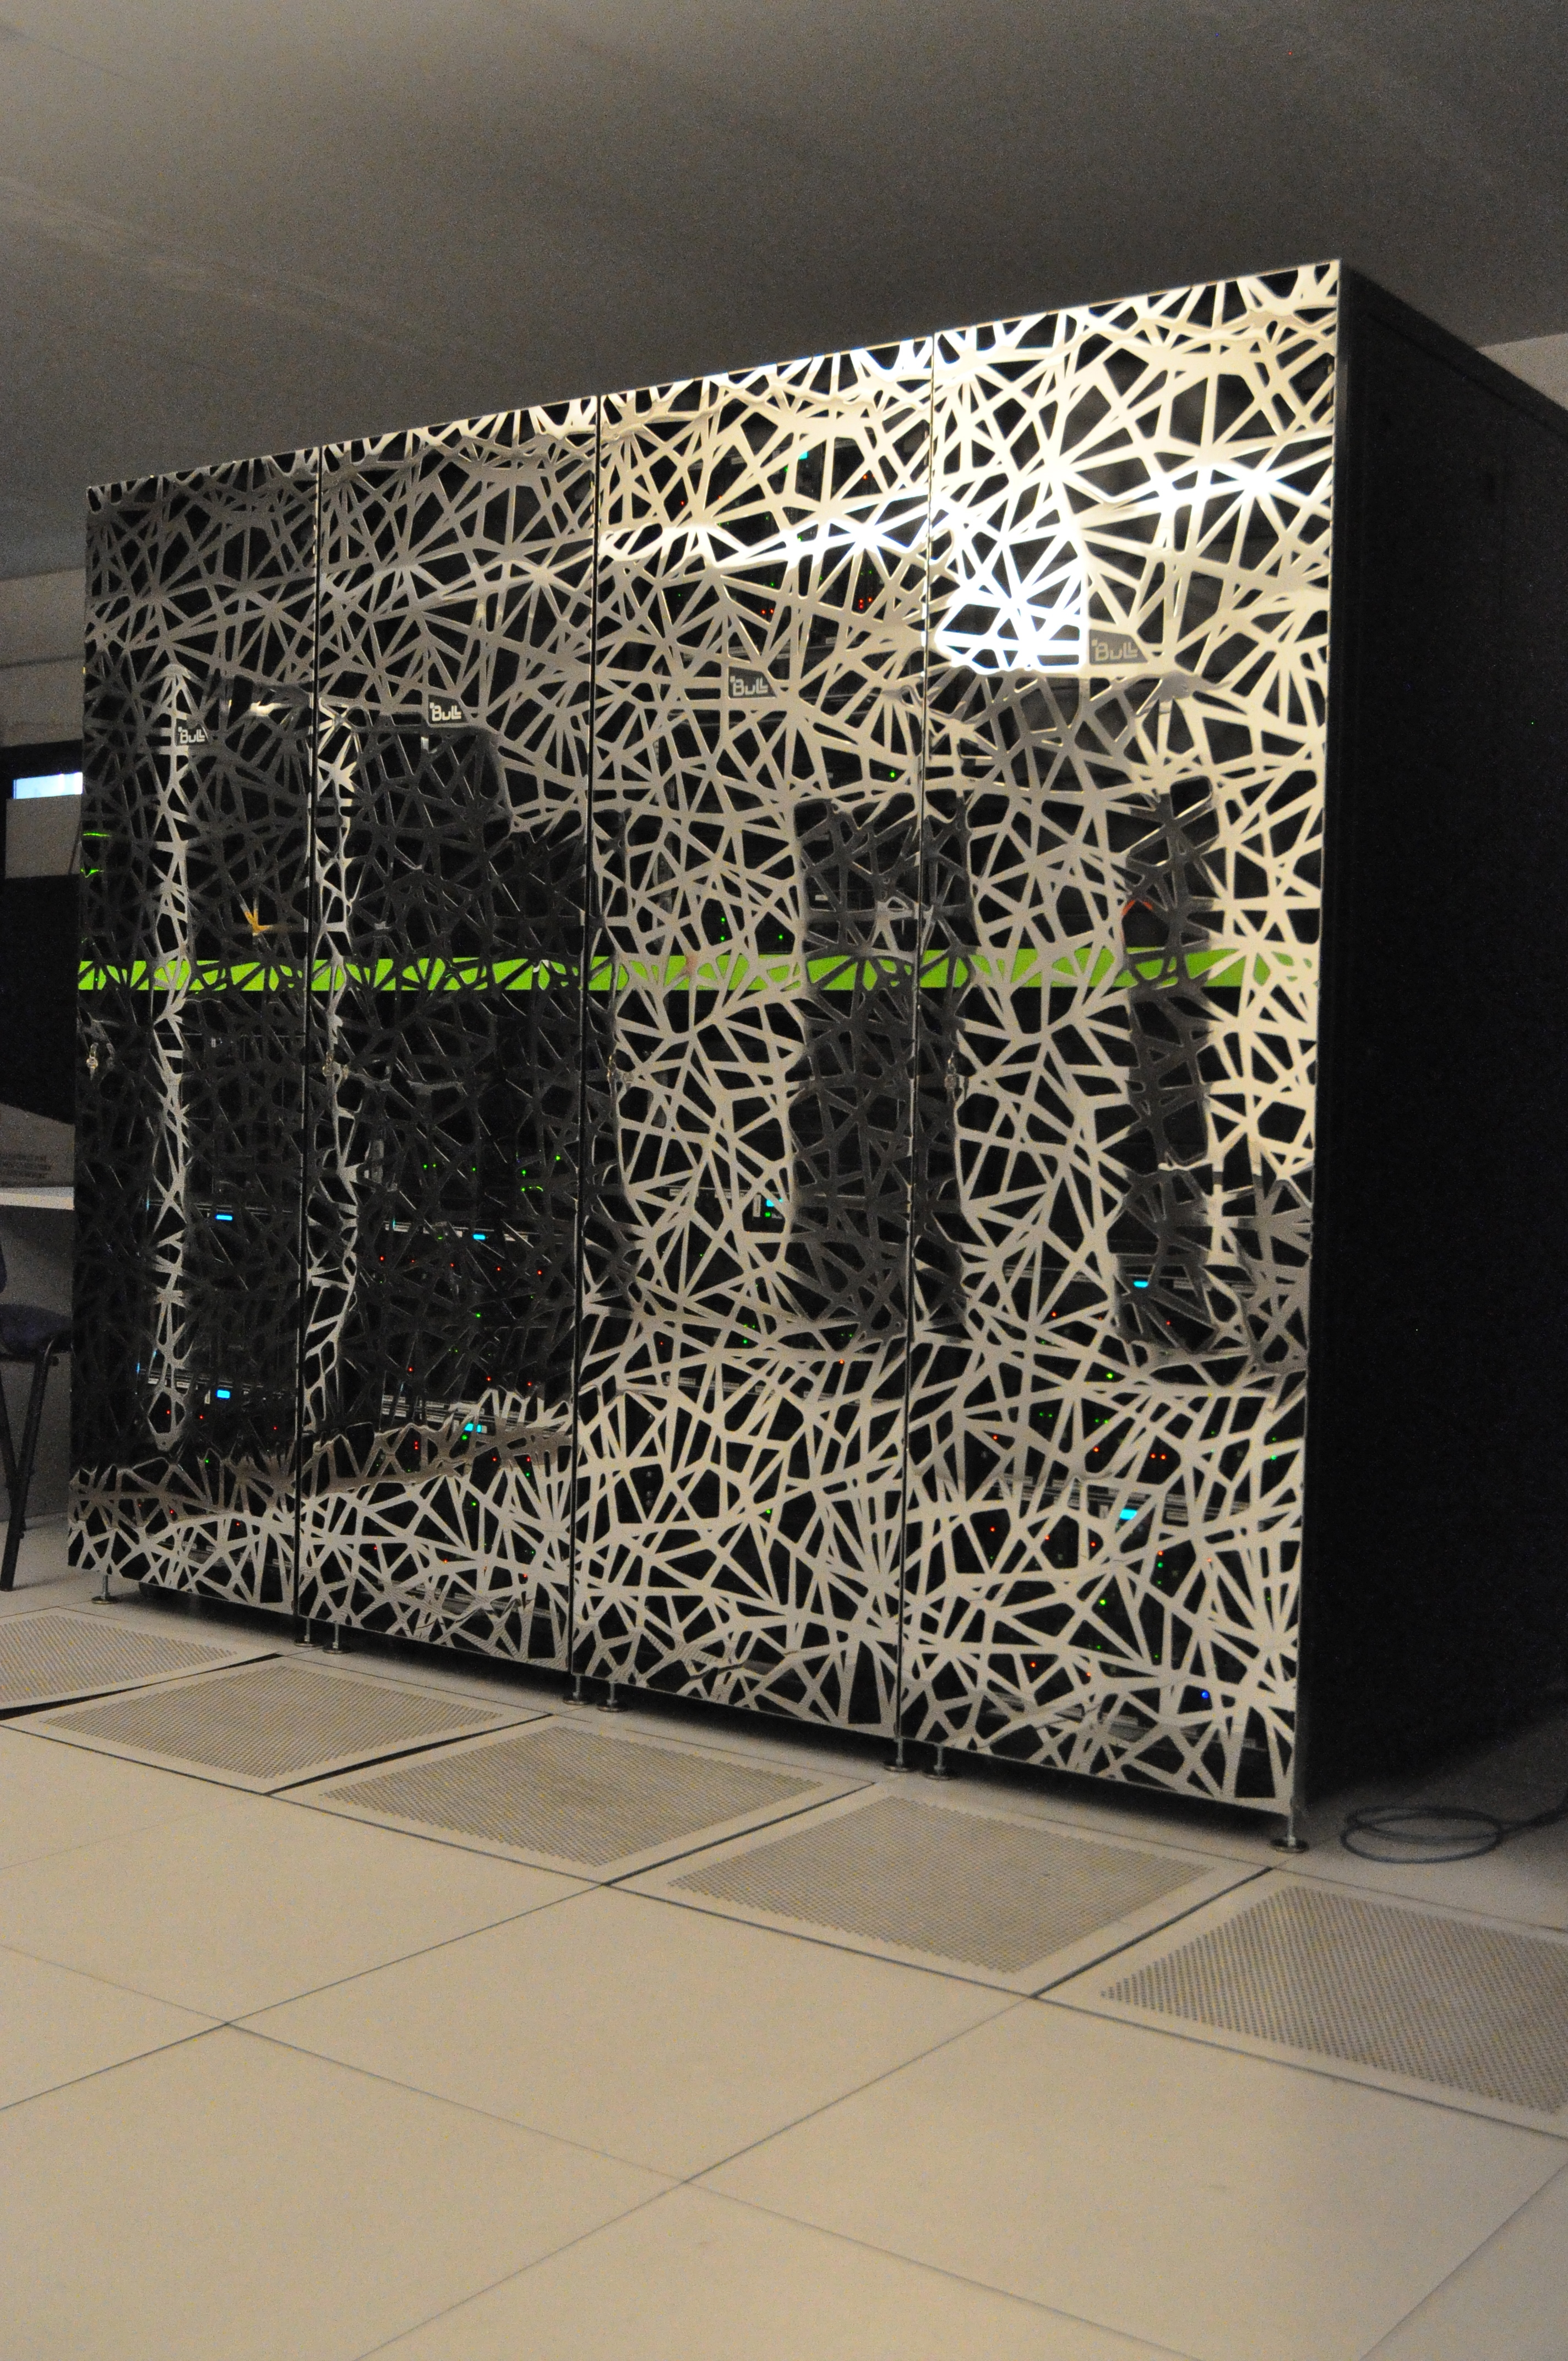
\includegraphics[width=.7\linewidth]{figures/neptune.jpg}
%    \caption{\label{fig:neptune}Neptune}
%  \end{minipage}%
%  \begin{minipage}{.5\textwidth}
%    \centering
%    \includegraphics[width=.9\linewidth]{figures/nemo.jpg}
%    \caption{\label{fig:neptune_node}Nemo}
%  \end{minipage}
%\end{figure}

\subsection{Métriques utilisées}
Le temps d'exécution pour calculer un point pour un pas de temps ($\mu s/it/p$). Plus cette valeur est basse, plus le code est efficace. 

\subsection{Performances séquentielles}
Dans cette partie, on s'interresse au programme testé et fonctionnel présenté dans la première partie. Avant de commmencer à profiler l'application, 3 cas ont été définis; ils permettent de couvrir une plus grande partie du code; en effet chacun de ces cas utilise des parties du code différentes:
\begin{itemize}
\item Cas périodique: le domaine de calcul est périodique
\item Cas non-périodique: dans ce cas, les frontières sont traitées
\item Cas symétrique: des méthodes de dérivations différentes sont utilisées
\end{itemize}

On part d'une taille de 20 points de coté (donc la taille du domaine est de $20\times20\times20$ points) et on l'augmente par pas de 50\%. Pour chacune de ces tailles de domaine, on réalise 20 itérations et on calcule la moyenne des temps par points de celles-ci.

%Une fois le programme testé et fonctionnel, j'ai commencé à étudier ses performances. J'ai, dans un premier temps, mesuré un temps de référence pour l'exécution de ce programme; compilation par défaut, donc avec l'option -O2.

\subsubsection{Vectorisation}
L'application est constituée de nombreuses boucles de calculs parcourant les tableaux contenant les variables conservatives. Il semble donc être un bon candidat pour la vectorisation. La vectorisation est présente sur les processeurs possédant des instructions SIMD (Single Instruction Multiple Data). On peut donc appliquer une opération sur plusieurs éléments à la fois au lieu d'un seul. Comme on peut le voir sur la figure \ref{fig:simd}, si on à une boucle calculant la somme de 2 tableaux, sans vectorisation, le processeurs réalisera une addition à la fois mais avec, il peut traiter plus d'éléments à la fois.


Sur LENOVO, le jeu d'instruction AVX2 est disponible, il permet de traiter des vecteurs de 256 octets, soit 4 nombre double précision. Si les boucles réalise beaucoup de calculs, on peut donc esperer diviser le temps par 4. Cependant, comme on peut le constater sur la figure \ref{fig:bench_scal_nemo}, la vectorisation n'a entraînée qu'un gain d'entre 18 et 25\% selon le cas. Grâce à Intel Advisor, qui permet d'analyser les boucles qui ont été vectorisées, il est possible de voir que:
\begin{itemize}
\item Certaines fonctions dans lesquelles le programme passe beaucoup de temps ne sont pas vectorisée à cause de dépendances, nottamment dans le calculs des gradients. Dans ce cas, on est dépendant de la méthode utilisée pour ces calculs et on ne peut pas forcer la vectorisation de ces boucles.
\item Beaucoup de petites boucles de calcul ne sont pas vectorisées. Ceci est dû à la structure de la mémoire du programme; tous les tableaux contennant des variables conservatives sont en réalité des sous-parties d'un plus grand tableaux. Lorsque des opérations sont effectuées sur ces tableaux, le compilateur assume qu'elle travaille sur un unique grand tableau et empêche donc la vectorisation au profit de la cohérence. Pour résoudre ce problème, il suffit d'indiquer au compilateur qu'il n'y a pas aliasing; on garantit ainsi qu'une zone mémoire ne peut être accédée que par un nom et que le programme ne dépassera pas les limites d'un tableau.
\end{itemize}



(memory bound)



\begin{figure}[h!]
  \centering
  \begin{subfigure}[b]{0.5\textwidth}
    \centering
    \includegraphics[page=1,scale=0.6]{gnuplot/bench_scalaire_nemo.pdf}
  \caption{\label{fig:bench_scal_nemo_nonper}}
  \end{subfigure}%
  ~
  \begin{subfigure}[b]{0.5\textwidth}
    \centering
    \includegraphics[page=2,scale=0.6]{gnuplot/bench_scalaire_nemo.pdf}
  \caption{\label{fig:bench_scal_nemo_sym}}
  \end{subfigure}
  \begin{subfigure}[b]{0.5\textwidth}
    \centering
    %\includepdf[pages={2}]{gnuplot/bench_scalaire.pdf}
    \includegraphics[page=3,scale=0.6]{gnuplot/bench_scalaire_nemo.pdf}
  \caption{\label{fig:bench_scal_nemo_per}}
  \end{subfigure}
  \caption{\label{fig:bench_scal_nemo}Temps par points des cas tests - LENOVO}
\end{figure}


\begin{figure}[h!]
  \centering
  \begin{subfigure}[b]{0.5\textwidth}
    \centering
    \includegraphics[page=1,scale=0.6]{gnuplot/bench_scalaire_neptune.pdf}
  \caption{\label{fig:bench_scal_neptune_nonper}}
  \end{subfigure}%
  ~
  \begin{subfigure}[b]{0.5\textwidth}
    \centering
    \includegraphics[page=2,scale=0.6]{gnuplot/bench_scalaire_neptune.pdf}
  \caption{\label{fig:bench_scal_neptune_sym}}
  \end{subfigure}
  \begin{subfigure}[b]{0.5\textwidth}
    \centering
    %\includepdf[pages={2}]{gnuplot/bench_scalaire.pdf}
    \includegraphics[page=3,scale=0.6]{gnuplot/bench_scalaire_neptune.pdf}
  \caption{\label{fig:bench_scal_neptune_per}}
  \end{subfigure}
  \caption{\label{fig:bench_scal_neptune}Temps par points des cas tests - BULL}
\end{figure}




\subsubsection{Alignement de la mémoire}
blabla marche pas

%\paragraph{durée=f(taille)}


\subsection{Performances parallèle}


%\subsubsection{Méthode de communication}
%Avant de comparer les méthodes de recouvrement, je me suis dans un premier temps interréssé aux méthodes de communication utilisées pour la première méthode (\ref{sec:}). Pour cela, j'ai comparer la durée passée dans des communications pour chacune des méthode et ceux pour différentes taille de grille.


%mesurer le temps d'exécution par point par pas de temps de chacune des méthodes pour différentes taille de grille.


%\subsubsection{Méthode de recouvrement}
%Je compare ici les 2 méthodes utilisée pour le recouvrement de domain présentées dans la partie précedente. Pour rappel: 





%\subsubsection{Décomposition du domaine}
%Le découpage du domaine est entièrement configurable par l'utilisateur, nous verons donc ici l'influence que ce découpage peut avoir sur le temps d'exécution du programme. 

\cleardoublepage
\section*{Conclusion}\addcontentsline{toc}{section}{Conclusion}

\paragraph{}A l'issu de ce stage, une version séquentielle et tridimensionnelle de NTMIX est fonctionnelle. Pour cela, j'ai moderniser le code de simulation, développé en Fortran 77, afin qu'il puisse utiliser la mémoire dynamique, facilitant ainsi son utilisation. J'ai ensuite modifié l'application afin qu'elle puisse traiter des simulations tridimensionnelles au lieu de bidimensionnelles.


\paragraph{}J'ai également développé une version parallèle de cette application pouvant s'exécuter sur des clusters de calculs grâce à MPI. Cette version permettra de traiter de plus grands maillage que la version séquentielle, permettant ainsi d'améliorer la précision des simulation. Cependant, au moment de ou j'écris ce rapport, je n'ai pas encore pu mesurer les performances de la version parallèle de NTMIX dans des conditions réelles d'utilisation. Ce point ferra donc l'objet de la fin du stage.




\paragraph{}Cependant, il est encore possible d'améliorer les performances de NTMIX. Par exemple, la quantité de mémoire utilisée peut encore être réduite. En effet, NTMIX a été pensé avec une approche mémoire statique; même si je l'ai modifié pour qu'il puisse utiliser de la mémoire dynamique, certaines parties du code devraient être entièrement réécrites pour mieux correspondre à cette nouvelle approche. 
NTMIX réalise également de nombreuses opérations sur des matrices et il serait donc intéressant d'étudier ses performances avec l'utilisation de librairies \textit{BLAS}, mais ces modifications nécessiteraient, comme pour de nombreux "vieux" programme scientifique, de réécrire entièrement le code et ne pouvaient donc pas faire l'objet de ce stage.



\appendix

\section{Annexe A}
\subsection{xxx}
\section{Annexe B}
\addcontentsline{toc}{section}{Bibliographie}
\bibliographystyle{unsrt}
\bibliography{biblio}
\end{document}
